 A three-dimensional rotation can be expressed as a sequence of angles - each associated with a rotation about a principal axis. We call this set of angles \emph{Euler Angles} \cite{lerios} \cite{goldstein} \cite{strauch}. The \emph{principal axes} are initially the $x, y$ and $z$ axes. The axes change as the rotation takes place but, nonetheless, stay perpendicular to each other. 

\begin{figure}[H]
	\centering
	\subfloat[Initial Principal Axes]{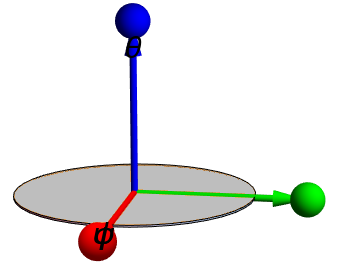
\includegraphics[scale=0.345]{initial}\label{fig:init}}%
	\qquad
	\subfloat[Rotation by $\phi$ about the $z$-axis (blue)]{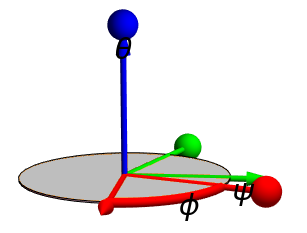
\includegraphics[scale=0.4]{phi_rotation}\label{fig:phirot}}%
	\\
	\subfloat[Rotation by $\theta$ about the new $y$-axis (red)]{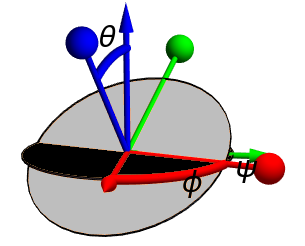
\includegraphics[scale=0.4]{theta_rotation}\label{fig:thetarot}}%
	\qquad
	\subfloat[Rotation by $\psi$ about the new $z$-axis (blue)]{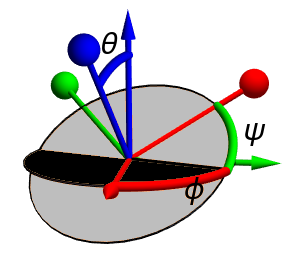
\includegraphics[scale=0.4]{psi_rotation}\label{fig:psirot}}
	\caption{\cite{strauch} \cite{goldstein} Rotation by Euler Angles}
	\label{eulerang}
\end{figure}

 As a demonstration, observe Figure \ref{eulerang}. Initially in \ref{fig:init}, we have the principal axes $y$ (red), $x$ (green) and $z$ (blue), each shown as arrows. We then rotate by an angle $\phi$ about the $z$-axis (blue) in \ref{fig:phirot}. Notice that as the rotation by the angle $\phi$ takes place, the $y$ (red) and $x$ (green) axes are displaced but remain perpendicular to $z$ and to each other. The displaced axes (each shown as a ball) now form a new set of principal axes from which we can then perform the next rotation in \ref{fig:thetarot}. Alternatively, we can visualize a rotation using a gyroscope as seen in Figure \ref{gyroscope}.

 \begin{figure}[H]
 	\centering
	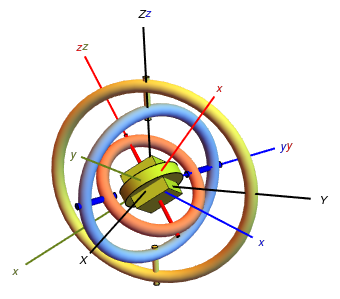
\includegraphics[scale=0.5]{gyro}
 	\caption{Gyroscope - Rotation about $y$ (green/yellow ring), rotation about $z$ (blue ring), and rotation about $x$ (red ring).}
 	\label{gyroscope}
 \end{figure}

Computing for a rotation using Euler angles requires $4\times 4$ matrices like the ones shown in Figure \ref{4x4}. 

\begin{figure}[h]
	\begin{align*}
			\Rx{R}{x}{\alpha} &=
			\begin{pmatrix}
				1 & 0 & 0 & 0 \\
				0 & \cos{\alpha} & -\sin{\alpha} & 0 \\
				0 & \sin{\alpha} & \cos{\alpha} & 0 \\
				0 & 0 & 0 & 1
			\end{pmatrix}
			&
			\Rx{R}{y}{\beta} &=
			\begin{pmatrix}
				\cos{\beta} & 0 & \sin{\beta} & 0 \\
				0 & 1 & 0 & 0 \\
				-\sin{\beta} & 0 & \cos{\beta} & 0 \\
				0 & 0 & 0 & 1
			\end{pmatrix} \\
			(a) & \text{Rotation by $\alpha$ in the x-axis} 
			& 
			(b) & \text{Rotation by $\beta$ in the y-axis}	
	 \end{align*} 
		 \begin{align*}
			\Rx{R}{z}{\gamma} &=
			\begin{pmatrix}
				\cos{\gamma} & -\sin{\gamma} & 0 & 0 \\
				\sin{\gamma} & \cos{\gamma} &  0 & 0 \\
				0 & 0 & 1 & 0 \\
				0 & 0 & 0 & 1
		 \end{pmatrix} \\
		 (c) & \text{Rotation by $\gamma$ in the z-axis}	
		\end{align*}
		\caption{$4\times 4$ Rotation Matrices about the Principal Axes}
		\label{4x4}
\end{figure}

Computations involving the matrices in Figure \ref{4x4}, however, are a bit tedious and require more elementary arithmetic operations \cite{lerios}. It's also more difficult to determine the axis and angle of rotation \cite{lerios}. Furthermore, this method is susceptible to a problem in mechanics known as the \emph{Gimbal Lock} \cite{jia}.

The gimbal lock is a phenomenon that occurs when two successive rotations are about the same axis, i.e., if two of the rings in \ref{fig:lock} coincide - resulting in a loss of one degree of freedom for the object being rotated \cite{jia}. Losing a degree of freedom 

\begin{figure}
\centering
\subfloat[A rotation by $\phi$ then $\psi$ about the same axis.]{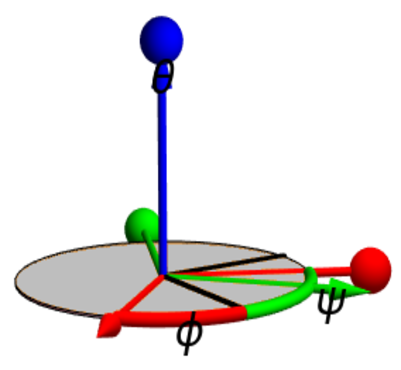
\includegraphics[scale=0.4]{gimbalLockrot}}%
\qquad
\subfloat[The blue and yellow/green rings coincide resulting in a loss of one degree of freedom.]{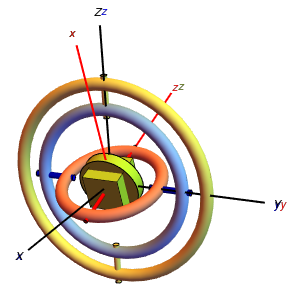
\includegraphics[scale=0.5]{gimbalLock}\label{fig:lock}}
\caption{Gimbal Lock}
\label{gimbal}
\end{figure}

%Ever since their discovery by William Rowan Hamilton in 1843, Quaternions have found extensive use in solving problems both in theoretical and applied mathematics - notably on the problem of 3D rotation.

Quaternions do not suffer from the gimbal lock. They are also found to be more compact - requiring less elementary arithmetic operations to perform rotation composition than rotation matrices \cite{lerios}. The axis and angle of rotation can also be easily deduced. Let $\vec{q}$ be the purely imaginary parts of the quaternion $q = a + b\ib + c\jb + d\kb $ ,i.e., $\vec{q} = b\ib + c\jb + d\kb$. It can be shown that $$\frac{\vec{q}}{\sqrt{b^2+c^2+d^2}} \text{ is the axis of rotation and }$$ $$\theta \text{ satisfying } \sin{\theta/2} = \sqrt{b^2+c^2+d^2} \text{ and } \cos{\theta/2} = a \text{ is the angle of rotation. \cite{lerios}}$$

Quaternions are used today in robotics, three-dimensional computer graphics, computer vision, crystallographic texture analysis, navigation, and molecular dynamics. 

Mathematicians have made advancements in developing the theory of Quaternions. Notably, as one of the central points of this topic, we look into the concept of a \emph{Quaternionic Matrix} and the implications it has on certain definitions that were already established in Linear Algebra. 

One such implication is the concept of a determinant in the context of quaternionic matrices. In linear algebra, we saw that we can extend the definition of the determinant to matrices with complex entries \cite{stamaria}. This is possible because the complex numbers are commutative under complex multiplication \cite{aslaksen}. 

Certain problems arise if we attempt to extend the classical definition to the quaternions because quaternions are not commutative under quaternion multiplication \cite{aslaksen}. In \cite{aslaksen}, Aslaksen revisits the properties we associate with determinants and gives three conditions called \emph{axioms} that should be satisfied in order for a definition of a determinant to be valid and useful:
\begin{enumerate}
	\item $det(A) = 0$ if and only if $A$ is singular.
	\item $det(AB) = det(A)det(B)$ for all quaternionic matrices $A$ and $B$.
	\item If $A'$ is obtained by adding a left-multiple of a row to another row or a right-multiple of a column to another column, then $det(A')=det(A)$.
\end{enumerate}

Over the years, several mathematicians have come up with different ways to define a determinant for quaternionic matrices - the Cayley determinant (by Arthur Cayley in 1845), the Study determinant (by Eduard Study in 1920), the Dieudonne determinant, and Moore's determinant. Aslaksen showed whether or not these different definitions satisfy the above conditions \cite{aslaksen}.

We will look at a particular problem that will require the concept of a determinant - that is, to determine whether or not the set of all $n \times n$ \emph{Skew-coninvolutory Quaternionic Matrices} (denoted by $\mathscr{D}_n(\HH)$) is empty when $n$ is odd. 

In \cite{stamaria}, Sta. Maria provided a simple proof to the fact that the set of all $n \times n$ skew-coninvolutory \emph{complex} matrices is empty when $n$ is odd. The method of proof involved using the determinant defined for complex matrices (which is not different from the classical determinant for matrices with real entries).

In this paper, we will discuss the theory behind quaternionic determinants - particularly, the Study determinant. We will then use the Study determinant to extend the result by Sta. Maria to the set of all skew-coninvolutory quaternionic matrices, i.e., we will show that the set of all $n \times n$ skew-coninvolutory quaternionic matrices is empty when $n$ is odd. 

\newpage
\section{List of Symbols}

\begin{itemize}
	\item $\Mr{n}$ - set of all $n\times n$ matrices with real entries.
	\item $\Mc{n}$ - set of all $n\times n$ matrices with complex entries.
	\item $\Mh{n}$ - set of all $n\times n$ matrices with quaternion entries.
	\item $\mathscr{D}_n(\C)$ - set of all $n\times n$ skew-coninvolutory matrices with complex entries.
	\item $\mathscr{D}_n(\HH)$ - set of all $n\times n$ skew-coninvolutory matrices with quaternion entries.
	\item $\cdet{ }$ - determinant of a matrix in $\Mc{n}$.
	\item $\rdet{ }$ - determinant of a matrix in $\Mr{n}$.
\end{itemize}